\section{Abstract}
This article describes an attempt to reproduce key findings of a study of murine hippocampal oscillations published in 2007 \cite{hentschke_muscarinic_2007}. Being a submission to the 'Ten Years Reproducibility Challenge', it focuses on the process of reviving the Matlab code underlying the analyses, particularly the neuronal signal processing toolbox created for the study and its follow-ups.

\section{Introduction}
\subsection{Neuroscientific background}
\label{subsec:background}
Neuronal activity in mammalian central nervous systems is often oscillatory. Intensity, frequency, and other characteristics of the oscillations are closely associated with behavior and arousal state. As this association suggests a functional role of oscillations, they have been studied extensively. One of the most conspicuous cases of behavior-dependent oscillatory neuronal activity occurs in hippocampus, a brain region pivotal for navigation and memory formation: prominent rhythms exist in the theta (4-12 Hz) and gamma (30-90 Hz) bands. 
Interestingly, the oscillations are coupled in a nonlinear fashion: the magnitude of gamma oscillations varies cyclically at theta frequency \cite{soltesz_low-_1993} (Fig.~\ref{fig:hip_oscill}). Such phase-amplitude coupling (PAC), also termed 'nesting' of oscillations, has been postulated to be important for memory formation and retrieval \cite{lisman_storage_1995, hyafil_neural_2015}.

A large body of research has shown that both theta and gamma rhythms depend on the neuromodulator acetylcholine, but before our study \cite{hentschke_muscarinic_2007} it had not been clear whether and how their PAC would change with cholinergic signalling. As a first step towards shedding light on this, we performed experiments on mice with extracellular multielectrode arrays implanted into area CA1 of hippocampus. Each extracellular electrode picked up local field potentials (LFPs) -- tiny, local, time-dependent changes in the electrical potential relative to a distant reference point (Fig.~\ref{fig:hip_oscill}B). The mice were behaviorally scored and the LFPs recorded for periods of ca.\ 90 min, including administration of a blocker of muscarinic cholinergic receptors 30 min into the experiments. 

\subsection{Code base and scope of reproduction}
The code presented here consists of two major parts. One is a toolbox of bespoke data crunching routines which performed classical time and frequency domain analyses. These were geared towards revealing spatial and temporal relations between signals from the different recording electrodes (crosscorrelations, coherence, etc.), with a focus on within-site phase-amplitude coupling. The 'main' function of this toolbox -- termed 'rmouse' -- integrated behavioral scoring data, partitioned the computational results according to the animals' behavior, and created summary figures for each recording (Fig.~\ref{fig:rmouse_workingstyle}). Also included were numerous post-processing routines with specific jobs like aggregation of data.

The other part of the code consisted of project-specific routines for statistical analyses of the data, and for the generation of publication-style plots.

The major focus here is on getting the toolbox and associated post-processing code to run with a Matlab version as recent as possible. Moreover, I attempted to reproduce those figures of the original study which conveyed the key finding of the paper, namely a reduction of PAC in the presence of muscarinic blockers (Fig.~\ref{fig:repro}).

\subsection{Expectations and results in a nutshell}
As Matlab code is generally quite backwards compatible, I was optimistic about overall success. The optimism was justified in terms of a general repeatability of the analysis; both toolbox and post-processing code could be brought into a functional state, and figures be created from the newly computed analysis results. However, data could only be retrieved for three of the five experimental animals of the original study, so the figures shown here are not exact reproductions, but must rather be seen as proofs of concept. 


\begin{figure}
	\centering
	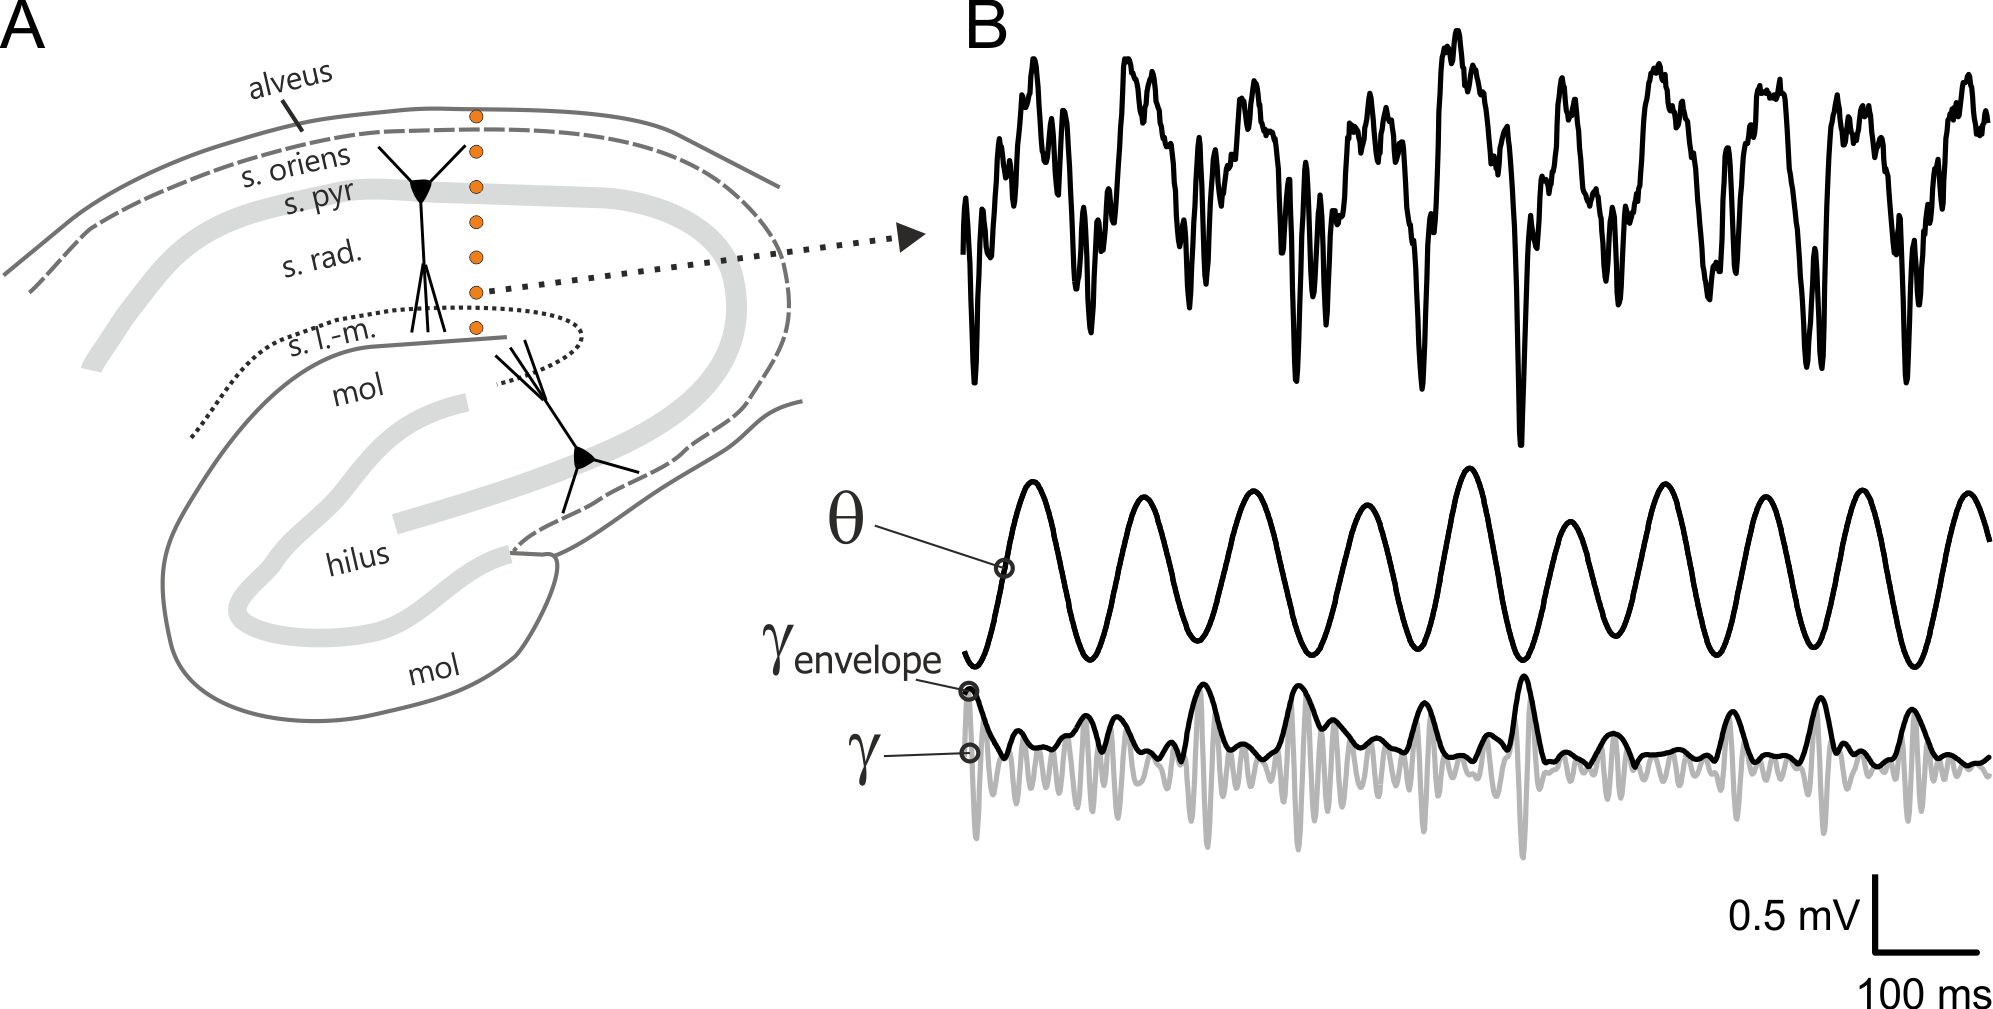
\includegraphics[width=0.9\textwidth]{figures/figures_tenYears_01.png}
	\caption{Theta and gamma oscillations, two prominent hippocampal oscillations under investigation in the original study. A, sketch of a section of rodent hippocampus and the location of the multielectrode recording arrays (orange circles). Shown are also two pyramidal cells with their basal dendrites in \textit{stratum oriens} and apical dendrites in \textit{strata radiatum} and \textit{lacunosum-moleculare}. B, wide-band local field potential data (top trace), and filtered versions (center and bottom, respectively) of a short stretch of oscillatory activity in the hippocampus of a mouse exploring its surroundings. Note how troughs of the slower theta oscillation (4-12 Hz) coincide with peaks in the envelope of the faster gamma oscillations (30-90 Hz).}
	\label{fig:hip_oscill}
\end{figure}


\subsection{Computational context}
% Describe the computational context: Which hardware was used to run the code? Which software infrastructure? Which constraints existed on software development? Which technical choices (language, libraries, ...) were made? Were reproducibility and/or re-usability important criteria? 
% About the original source code: Was it published? Was it archived somewhere? Was there a license for it? 

I developed the largest part of the code during a postdoctoral stay 2003-2005 in the laboratory of Robert A. Pearce (University of Wisconsin at Madison). The core of the analysis strategy had been devised by Matthew I. Banks (also UW Madison), who had also implemented a first version in a spreadsheet-cum-script language (Origin). Due to limitations inherent in the language it was decided to implement and extend the analysis in a more versatile language. Matlab was the natural way to go, as it was (and still is) the standard programming environment in many electrophysiology laboratories, and I had used it extensively before. In our original study \cite{hentschke_muscarinic_2007}, Matlab versions 6.5 - 7.4 (R13 - R2007a) were used. For later projects, the code has been continuously adapted to Matlab versions up to 7.9 (R2009b), after which it lay dormant. Various Matlab toolboxes were required: most importantly, the Signal Processing Toolbox; depending on the exact post-processing routines, the Curve Fitting and Statistics Toolboxes were also required. 

A pivotal issue for the project, and in general for any data-focused undertaking, was the import of raw data. The time series data existed in a proprietary format, the Axon Binary Format (ABF), in which each data point is stored as a 16-bit integer. A function for efficiently importing data of this format into Matlab did not exist. Although the software package provided by the vendor (former Axon Instruments, now Molecular Devices) allowed an export of the data into text format, this was not considered practical (tedium involved in manual conversion, inflation of data size). Hence, I wrote a routine for importing raw data in this format into Matlab and submitted it to the MathWorks Central File Exchange \cite{hentschke_abfload_nodate}. Initially considered a spin-off of minor importance, this routine and its upgrade \cite{collman_fcollmanabfload_nodate} found a widespread distribution in the neuroscience community, and also sparked implementations in other languages \cite{caldwell_abfload_nodate, harden_swhardenpyabf_nodate}. An ironic twist is that the more fail-safe way of implementing a data importing routine for the windows operating system, namely code employing Molecular Devices' dynamic link library (DLL), would have made sense at the project's start in 2003, but has since the introduction of 64-bit versions of Matlab been rendered impractical by the limitation of this DLL to 32 bit (confirmed via an exchange with Molecular Devices Customer Support in December 2019). Readers further interested in this topic may want to consult the "Unofficial Guide to the ABF File Format" by Scott Harden \cite{harden_scott_w_unofficial_nodate}.

As all code was written in pure Matlab, and data import had been solved within Matlab, there were no extraneous dependency issues.

Although reproducibility of the study results was not an imminent concern to me back then, reusability of the code had definitely been an important design aspect early on. Series of experiments with a similar setup were in the pipeline, and given the limited term of my stay it was clear that the code would also be used by my colleagues \cite{perouansky_amnesic_2007, hentschke_altered_2009, balakrishnan_midazolam_2014}. Therefore, I wrote a manual with illustrations, with the intent of providing sufficient information for lab members familiar with the scientific background to find their way through the code. I also commented the code prolifically, especially the scripts calling the toolbox functions. The source code has never been properly archived or published, except for the data importing routine (until the reproducibility challenge came along) for two reasons: first, I considered it too specialized and tailor-made to be of much use for other groups. Second, making the toolbox open access would have required making it more user-friendly and extending the documentation substantially. Absent an academic reward system for such efforts not only for myself but also the hosting lab, I considered the necessary investment of time inappropriate.

I developed the code without any kind of version control worth the term, and left it 'as is' on my then machine in the laboratory. The toolbox's core code was in one dedicated directory, but auxiliary code was scattered throughout my Matlab code base, which of course also contained a great deal of unrelated code. I never saw the necessity of properly packaging the code: it would not be published, and almost all auxiliary functions employed by the toolbox were quite general and therefore also part of other (and future) programming projects. So, my justification for this practice was to avoid redundancy and the usual problems associated with maintaining multiple copies of code.

Towards the end of my stay in the laboratory, I simply mirrored my Matlab directory on other users' machines to get the toolbox to run there. After I left, I developed it further and adapted it to the needs of the subsequent projects, which went on for quite a while. 

Hardware was an issue, albeit an uncritical one. The analyses were run on 32-bit Windows PCs with 4 GB of RAM and not-too-bad Intel Pentium processors available at the time (more precise specs are not known anymore). The electrophysiological signals were sampled at ca. 1000 Hz from up to 16 channels and typically lasted for 30 minutes; the resulting individual raw data files occupied less than 100 Mb on disk. Their size in RAM, after conversion from 16-bit integers to the default 64-bit floating type in Matlab, posed no critical challenge. However, the code also implemented the creation of surrogate time series. Dealing with these, as well as multiple filtered copies of the data in RAM in parallel required some thought-through strategies and juggling with computer resources, and was taxing for the CPU. Yet, even full-blown analyses of the whole data set were accomplished overnight.


\section{Retrieval of the software}
% Was it easy to find a copy of your source code? 
% Was it easy to locate and setup the dependencies? 
% Provide a list of all dependencies (libraries but also tools such as compilers). 

Retrieval of the source code was easy; in fact, most of it did not have to be retrieved. As code files are ridiculously small even by the standards of the mid-2000s, I generally leave them on the hard disks of the computers in my hands. The hard part was figuring out the organization of the code files. There were the toolbox folder, still in my Matlab code base, and the folder containing code files for generating the publication figures. Localizing both required just a few minutes. I was also aware that several auxiliary functions, including the data-importing function, were outside the toolbox folder but inside my Matlab code base. However, I forgot that back then I placed scripts defining analysis parameters for each individual data file in yet a different location: namely, in the root folder for the raw data, as well as the subfolders therein. Only after I tried to run the first analysis step did I realize this.

\section{Execution}
% Describe what you did in order to run the software today.
% • Did you succeed in running the software in a modern computational environment? Or did you have to search for old versions of tools and libraries? 
% • Describe the computational environment of the reproduction: hardware, operating system, compiler versions etc. 
% • Did you have to modify the software in order to make it run today? 
% • Were the original instructions that came with the software sufficient, or did you have to modify or extend them? 
% • How close were the results you got to the originally published ones? Include the replicated data table and figure, as we do in other ReScience articles. 
% If you had to make any modifications to the software or to the instructions that were supplied with it, try to describe which competence another researcher would need in order to do the same work. Would a general familiarity with your programming language and environment have been sufficient?

Reproduction was performed on a PC with Windows 7 and Matlab R2020a with the Signal Processing, Statistics and Machine Learning, and Parallel Computing Toolboxes installed. The PC had 32 GB of RAM, ample space on both hard disk and solid state drive, an Intel Core i7-4770K CPU with four physical cores, and an nvidida GeForce GTX1060 graphics card.

Reproducing data analysis including selected figure panels of the original paper required several processing steps. 
I started with the first step -- processing the raw data -- by trying to locate the scripts which defined the analysis parameters for each individual file to be processed. After finding only one, I read the manual, and realized that both the majority of the data and data-specific scripts were missing, contrary to my first cursory impression when entering the challenge. Thanks to the efforts of a former colleague (acknowledgements) I was able to retrieve six complete sets of data and data-specific scripts from three of five experimental animals used in the original study. With these available, I finally remembered how the toolbox was supposed to work.

Before actually trying to run it, I assembled all code files I could identify at this stage as belonging to the project into a directory structure such that submitting the code to a repository would be possible. Next, I ran a dependency analysis on the main function of the toolbox and could identify a number of additional code files that were missing. After copying these to the project directory, I excluded my general Matlab code base from the path. Then, I tried in earnest to start number crunching. It took me about three hours to get the analyses to run on three experiments (two data files each). The adjustments required were, in order of severity:

\begin{enumerate}
	\item Retrieval of functions that were still missing from my general Matlab code base (about two dozen of files).
	\item 'Downgrading' auxiliary functions which had been in my general code base and together with it had evolved over time to the point of being incompatible with the toolbox.
	\item Updating code to be compatible with the recent version of Matlab.
\end{enumerate}

I was shocked to learn how many of the required functions I had to retrieve from my '\_legacy' folder. Had I not exerted caution in getting rid of code and instead deleted them, I would have spent hours on end to recapitulate what they were supposed to do, and possibly given up. A pleasant confirmation of expectations was the little effort I had to spend adapting the code to the most recent Matlab version. Essentially, all I had to do was write a wrapper for function \texttt{diag}, which did not accept cell arrays as inputs anymore. Surprisingly, graphics, including one very simple GUI, worked without hiccups; thanks to a major revision of graphics in R2014b, it also produced more aesthetically pleasing figures. 

Moreover, with little effort, it was possible to run number crunching in an embarassingly parallel way using \texttt{parfeval}. This, as well as moving the data to a solid state drive, cut down processing time from a baseline of 152 min to a very agreeable 66 min (three experimental subjects, two recordings each, 100 instances of surrogate data generation each). Although exact numbers are impossible to come by, my estimate is that the combination of recent software and more modern (certainly not recent) hardware sped up the computations by a factor of at least eight. Yet more speedup would have required fundamental re-coding of the toolbox.

\begin{figure}
	\centering
	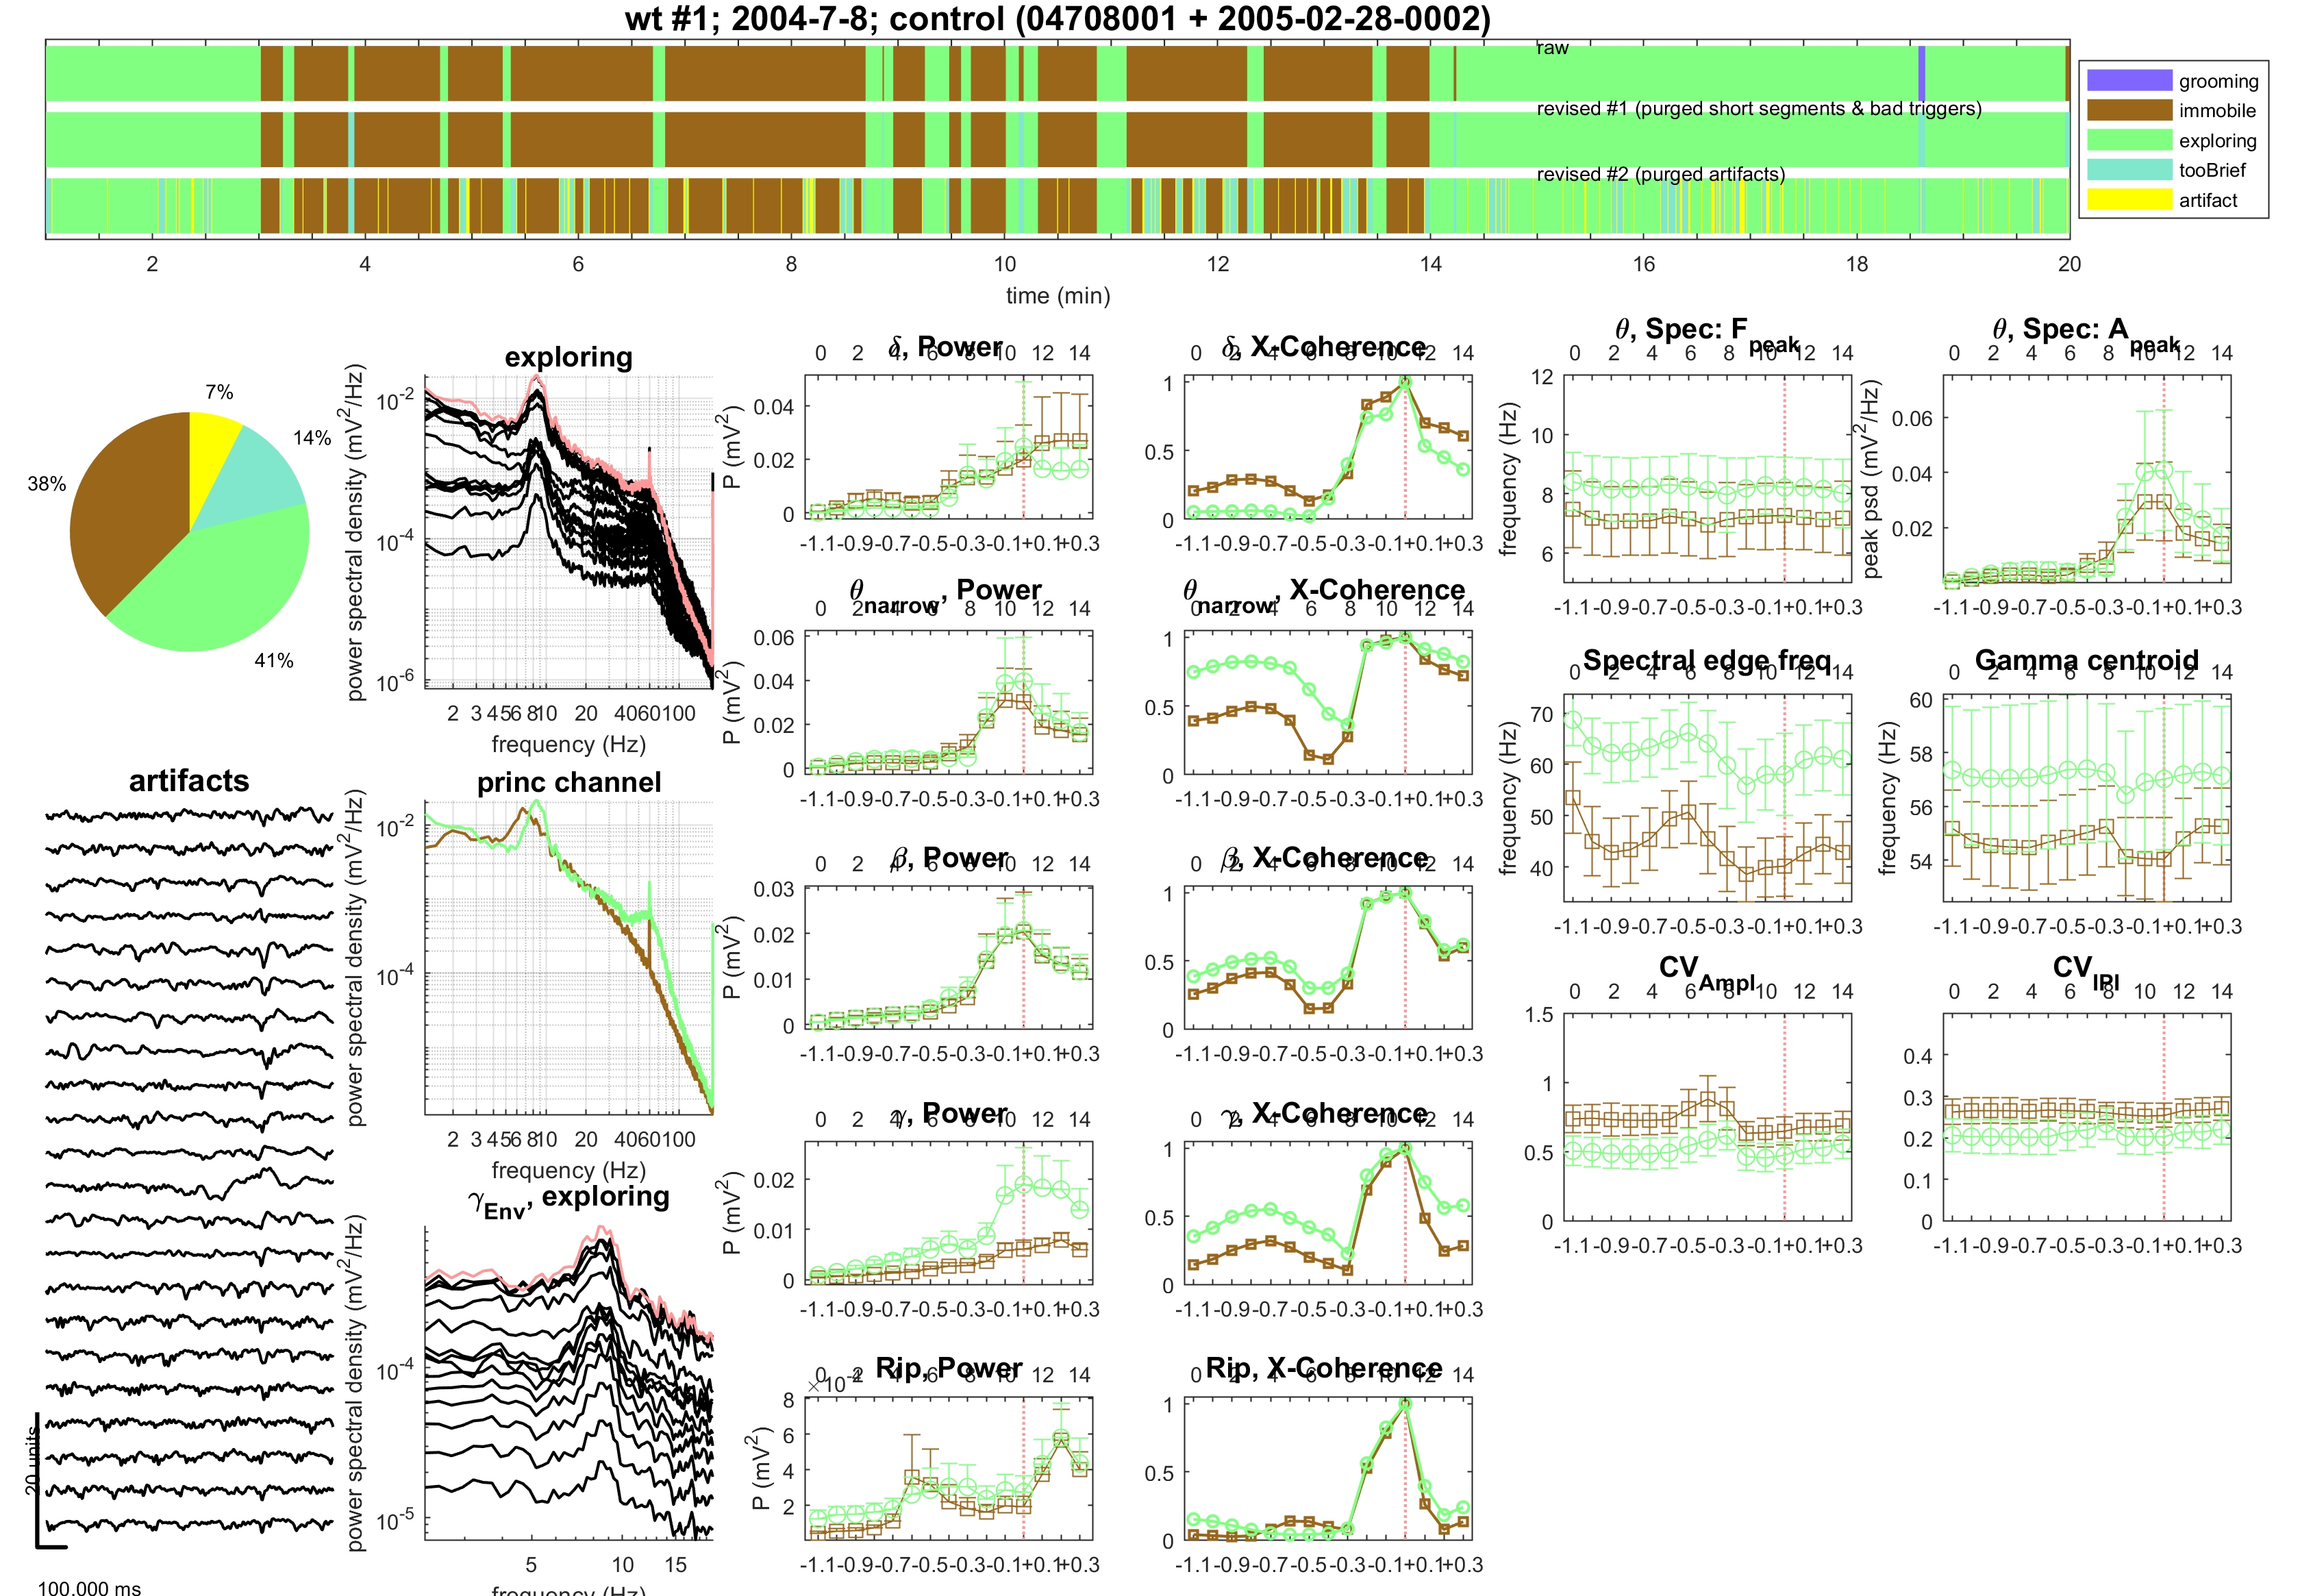
\includegraphics[width=0.9\textwidth]{figures/example_summaryFig_rmouse.jpg}
	\caption{Example of a summary figure produced by the rmouse toolbox from one of the analyzed data files. These summary figures were meant to provide a quick overview of the data and a glimpse at the computed quantities. The top panel and pie chart on the left illustrate the temporal sequence and proportions of time spent in various behavioural states, respectively, and also quantify recording periods unsuitable for analysis. Examples of data segments considered artifacts are depicted on the left, below the pie chart. All other panels show the results of spectral and time domain analyses.}
	\label{fig:rmouse_workingstyle}
\end{figure}

The next task was aggregating the data from the different experiments, and (re-)producing selected figure panels of the original study. Numerous scripts for various visualizations of the results existed; as these were not strictly documented and kept up to date, a trial-and-error period of identifying key pieces of code responsible for producing the plots ensued. Apart from this, and on top of adjustments similar to those required for the toolbox, I expected two additional problems here. First, the original code made use of the Curve Fitting Toolbox, which was not at my disposition now. Second, code producing 'Christmas Tree' plots -- adorned horizontal bar plots often featuring a coniferous shape (Fig.~\ref{fig:repro}) -- featured low-level graphics commands. Due to substantial changes of Matlab graphics in the interim, I knew that this code would have to be modified.
Both challenges proved surmountable. For the simple fits of 1D data, I used function \texttt{fitnlm}, and refurbished the affected code accordingly. The function producing the horizontal bar plots could also be updated without major pains. Following these fixes, key findings of the original study could be reproduced, albeit only with said partial data (Fig.~\ref{fig:repro}). All other figure panels featuring above-mentioned horizontal bar plots could be reproduced with the same data base by  changing the name of a target variable in a script and adapting the curve-fitting code (data not shown).

\begin{figure}
	\centering
	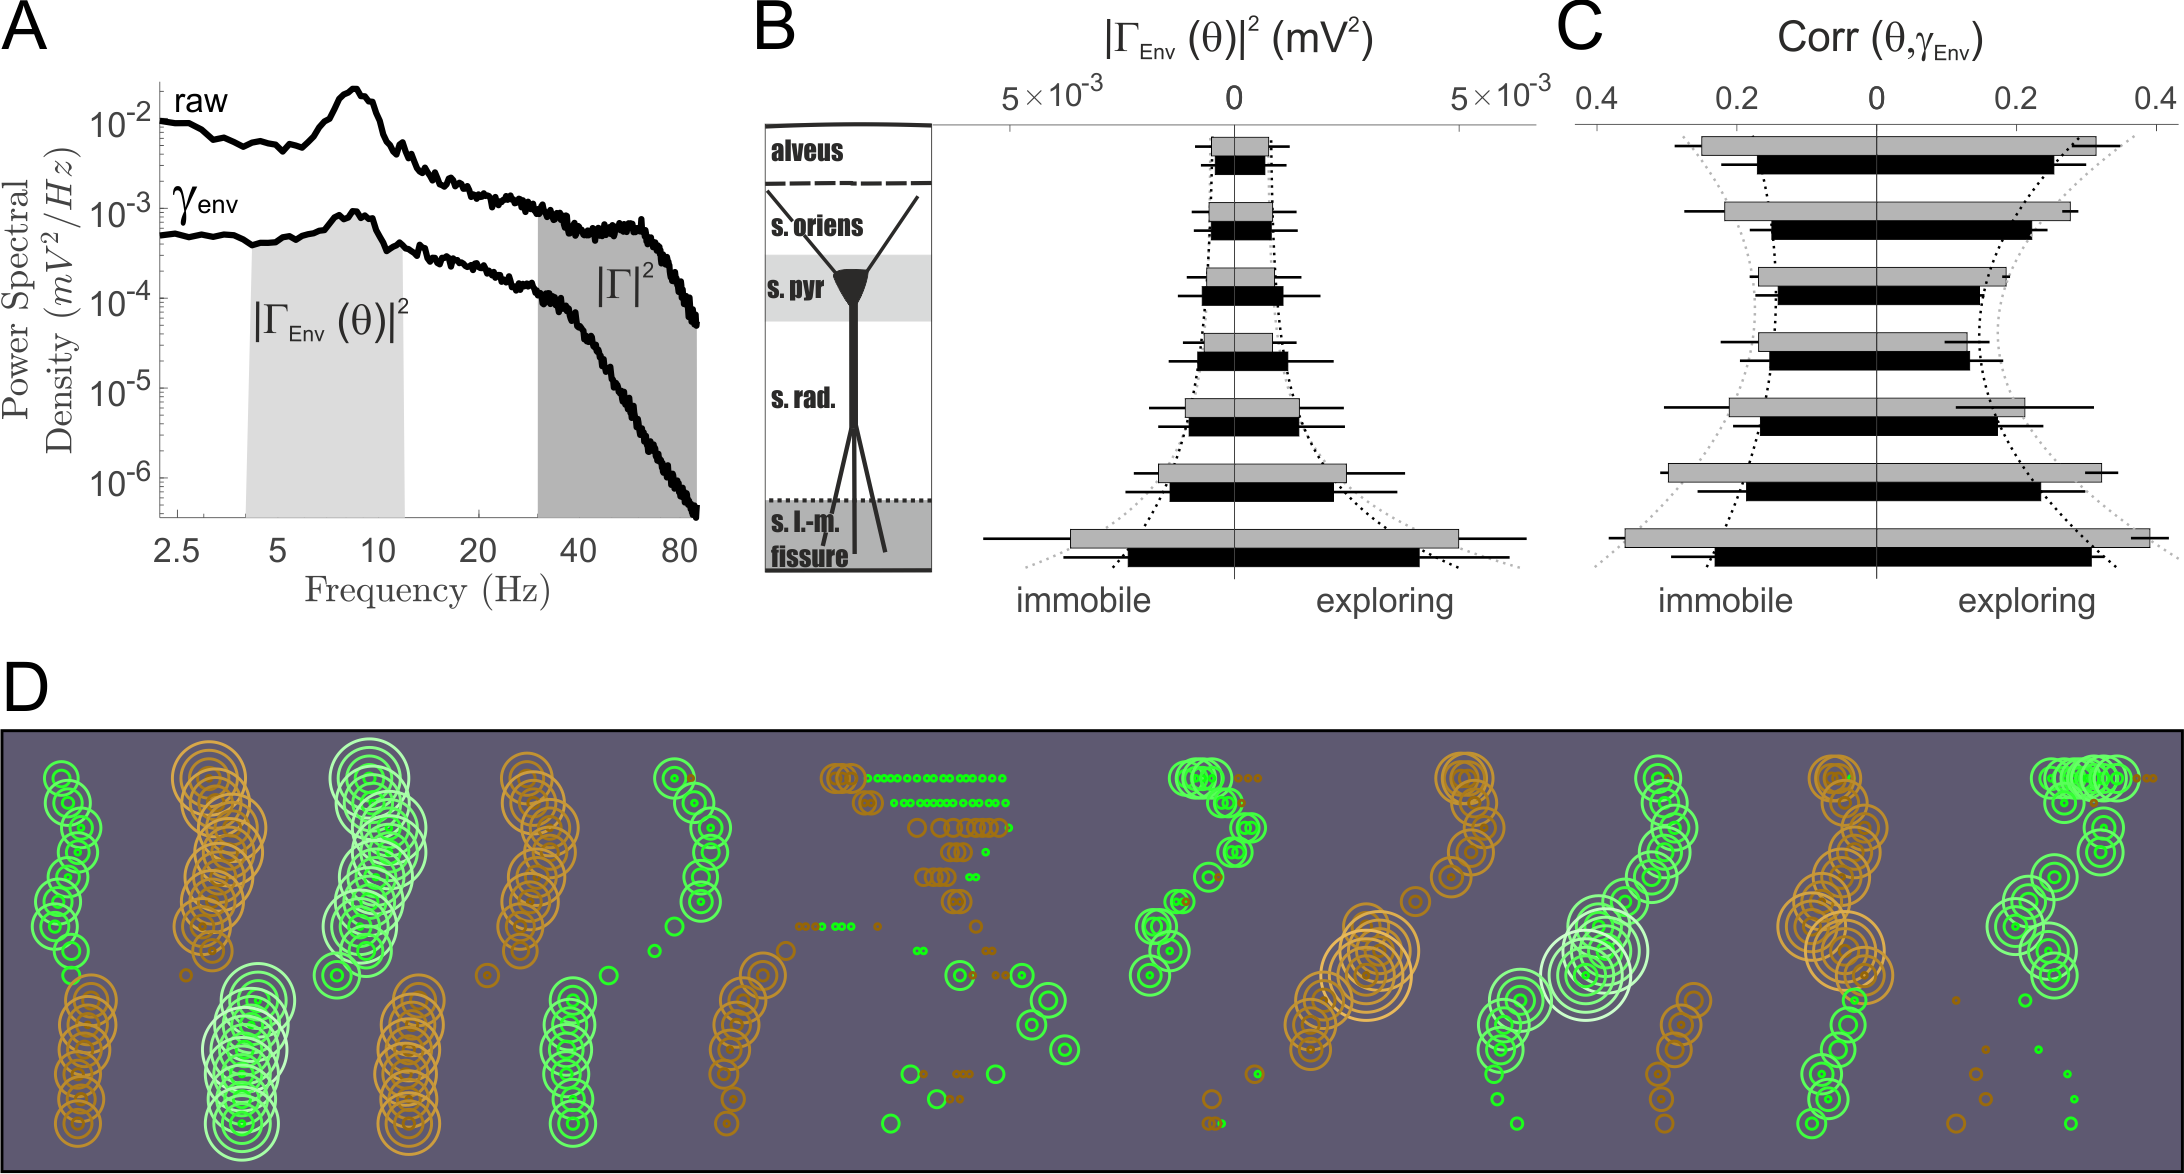
\includegraphics[width=0.9\textwidth]{figures/figures_tenYears_02.png}
	\caption{Reproduction of key findings. A, exemplary power spectral densities of the wide-band LFP ('raw') and of the gamma envelope of the LFP recorded at the hippocampal fissure. The light shaded area corresponds to the power of the gamma envelope in the theta range; the gray area represents the power of the gamma oscillations. This graph corresponds to Figure 5B in the original paper. B, laminar profile of the power of the gamma envelope in the theta band for immobile and exploring  animals (three of five from which data could be retrieved). The vertical position of the bars illustrates the location of the recording sites underlying the data. Gray, control; black, with the muscarinic blocker atropine. Error bars are standard deviations. Dotted lines are exponential fits to the data. This graph corresponds to Figure 5C in the original paper. C, laminar profile of the crosscorrelation between theta and the gamma envelope. Same conventions as in B apply. Dotted lines are polynomial fits (order 2) to the data. This graph corresponds to Figure 7A in the original paper. D, artistic rendering of theta oscillations, illustrating their highly dynamic nature. Time runs horizontally from left to right. Each set of concentric rings represents a theta peak (green) or trough (orange) detected on each of the 16 electrodes spanning hippocampus (and a trifle of the surrounding tissue). The more rings in a set, the stronger the normalized peak or trough amplitude (as amplitudes differ strongly between the layers, they were normalized for each recording electrode separately). The orientation of recording sites is as in the sketch in B (topmost row corresponds to \textit{stratum oriens/alveus}). On average, there is a phase lag of almost half a theta period between the layers harboring the apical and basal dendrites of the pyramidal cells, but individual theta 'beats' are very variable. The increase of such variability in the presence of atropine (data not shown) is a major cause of the deteriorated coordination between theta and gamma (as shown in C). Modeled after Figure 9A in the original paper.}
	\label{fig:repro}
\end{figure}



\section{Conclusion and personal evaluation}
During my last years in academia, I focused increasingly on professional programming, and eventually left academia in 2019 to work as a Data Scientist. Having along the way picked up at least a modicum of formal software education, my opinion on my original source code is mixed. 

On the positive side, I commented the code heavily, particularly the scripts which other users of the code were to use. Later on, I also spent a considerable amount of time on the documentation. A crude form of logging was implemented. Moreover, I had a knack for making code run fast, and consider some aspects of the implementation valid even today.

However, a few of my past code design choices strike me as odd now, to say the least. First and foremost, this is above-mentioned liberal dispersal of code files across my entire code base, and the placement of scripts defining parameters in data directories. The cascades of scripts required for running analyses with the toolbox required immersion into the code, and could have been replaced by a more user-friendly graphical user interface. For post-processing, there had been a proliferation of poorly documented and partly redundant helper or plotting functions. Over time, 13 (thirteen) variants of a 'combine\_X'-function had accumulated, the job of which was to assemble the results of the computations by the toolbox. Moreover, I would have compartmentalized the toolbox code much more. Finally, for a toolbox of this scope, more time should have been devoted to the documentation. All things considered, I believe that resurrecting the code would have been very arduous for anyone else, even a Matlab expert, due to a dearth of documentation.

Yet, I view these deficiencies in context. As a scientist-cum-programmer, one also has the science to do, not to mention actually making sense of the analysis results and writing papers about them. As mentioned before, spending a large amount of time on the documentation would have been hard to justify. Moreover, like many of my former colleagues, I was a self-taught programmer essentially without formal computer science education, so most of my design choices were not based on traded wisdom, but self-accrued, patchy knowledge. 

My former self was certainly not alone in this position, as academia in general seems to be a fertile ground for 'organically home-grown' code that may or may not be 'good enough' to publish \cite{barnes_publish_2010}. It is heartening to see that programming scientists are increasingly given a hand in producing reproducible and efficient code \cite{wilson_good_2017}.

\section{Acknowledgements}
I owe profound thanks to Claudia Holt, Section of Experimental Anesthesiology, University Hospital of Tübingen, who unearthed the data for this study. Many thanks also go to Matthew I. Banks for discussions of the manuscript, and to Robert A. Pearce for consenting to the publication of the code.